%%% Local Variables: 
%%% mode: latex
%%% TeX-master: t
%%% End:

\documentclass[a4paper, 10pt]{article}

\usepackage[utf8]{inputenc}
\usepackage{hyperref}
\usepackage{enumerate}
\usepackage{multirow}
\usepackage{wrapfig}

\usepackage{fancyvrb}
\DefineVerbatimEnvironment{code}{Verbatim}{fontsize=\small}
\DefineVerbatimEnvironment{example}{Verbatim}{fontsize=\small}

\usepackage{graphicx}
\usepackage{caption}
\usepackage{subcaption}
% \usepackage[margin=2cm]{geometry}
\usepackage[backend=bibtex]{biblatex}
\addbibresource{references.bib}

\title{Software Reengineering\\
       Assignment 2}
\author{Joey Ezechi\"{e}ls (1338994) \and Volker Lanting (1513273)}

% % Implement x.yy numbering scheme for subsections
% % where yy is *always* a 2-digit number
% \makeatletter
% \renewcommand\thesubsection{\thesection.\two@digits{\arabic{subsection}}}
% \makeatother

\begin{document}
\maketitle % Doesn't count towards the total number of pages
\pagenumbering{roman}

\newpage
\tableofcontents % Doesn't count towards the total number of pages

% \newpage
% \section{Introduction}
% \label{sec:introduction}

\newpage
\pagenumbering{arabic}
\section{Introduction}


\section{Refactoring}
We have chosen to refactor the JmeSystem, 
because it's a good example of a S.O.L.I.D. SRP violation.
This means it does too much and therefore its afferent coupling is higher than it has to be.
The afferent coupling of JmeSystem is diplayed in Figure~\ref{fig:system-incoming}.
Changes in the JmeSystem are therefore harder to make without breaking other code,
which is bad for maintainability.

	The system itself uses a delegate, so the involved classes are JmeSystem, JmeSystemDelegate and JmeDesktopSystem from the com.jme3.system package, and JmeAndroidSystem from the com.jme3.system.android package.

	We plan to write an extensive testsuite for these classes, which will be used to record their behaviour.
	Then we will proceed to split the functionality in to smaller chunks with a more defined responsibility.
	By introducing interfaces for each of these chunks, we will further increase extendability and reusability.
	As these chunks can then be easily swapped and shared between different system types.
	Our proposed decomposition of JmeSystem into parts with a single responsibility and the resulting decrease in afferent coupling
	can be seen in Figure~\ref{fig:system-decomposition}.

\begin{figure}[!hb]
\hspace*{-20mm}
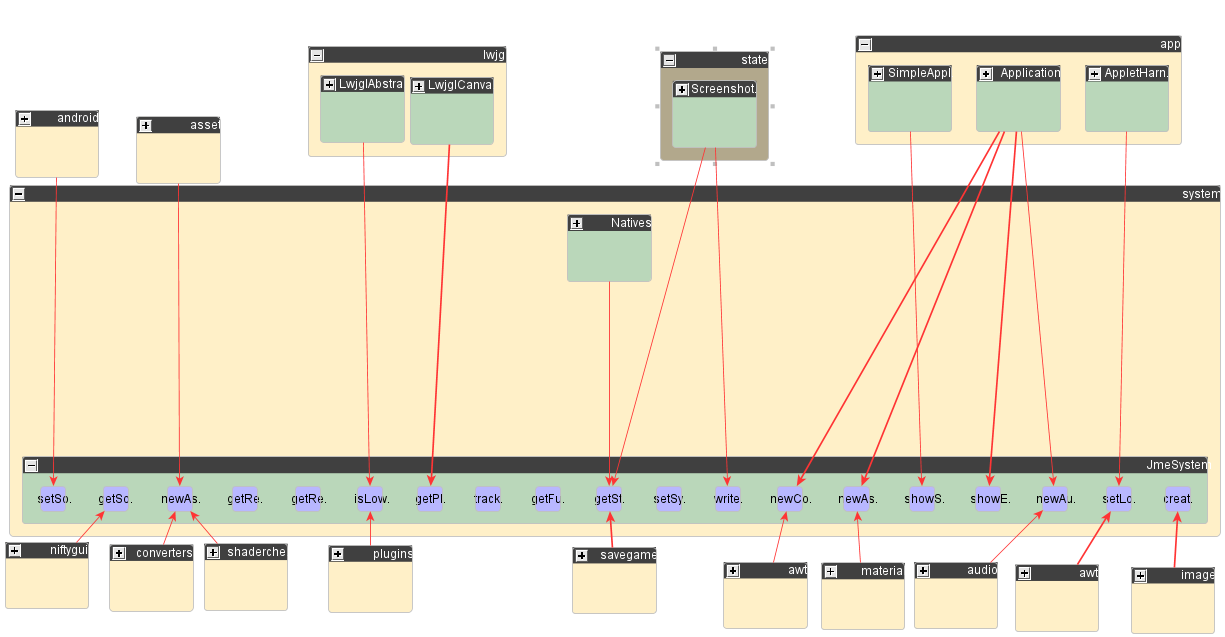
\includegraphics[width=1.3\textwidth]{figures/jme-system-deps.png}
\caption{The incoming dependencies of the JmeSystem. It is clear that these dependencies can be split up into smaller groups.}
\label{fig:system-incoming}
\end{figure}

\begin{figure}
\begin{subfigure}[b]{0.6\textwidth}
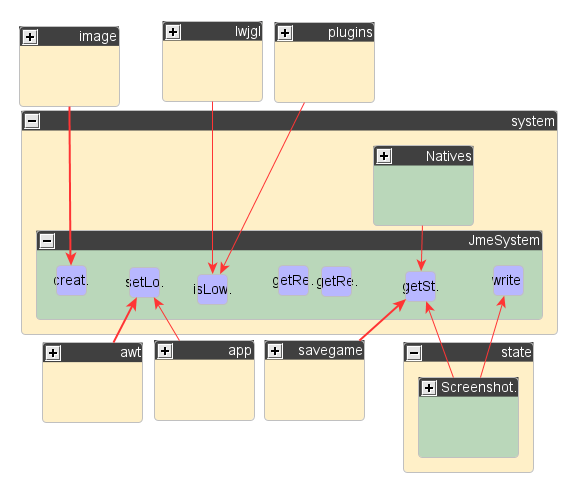
\includegraphics[width=\textwidth]{figures/jme-system-io-part.png}
\caption{This subsystem's main focus is IO, as the lowPermissions state is mostly related to which IO operations are allowed.}
\label{fig:system-io-incoming}
\end{subfigure}
~
\begin{subfigure}[b]{0.4\textwidth}
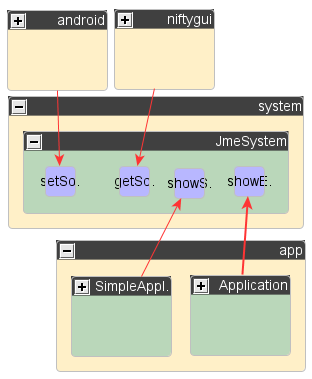
\includegraphics[width=\textwidth]{figures/jme-system-dialog-part.png}
\caption{The incoming dependencies of a sub part of JmeSystem, which we believe has the responsibility of dealing with Dialogs.}
\label{fig:system-dialog-incoming}
\end{subfigure}

\begin{subfigure}[b]{0.6\textwidth}
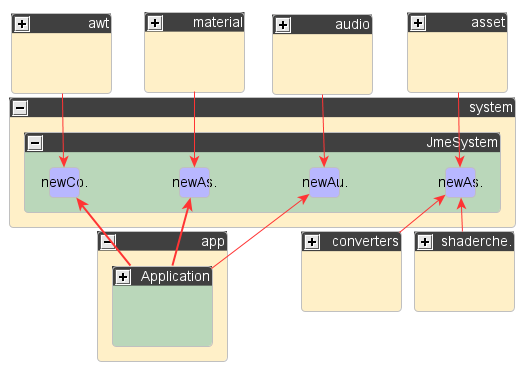
\includegraphics[width=\textwidth]{figures/jme-system-factory-part.png}
\caption{This subsystem's main focus is creating new instances of certain sytem related classes.}
\label{fig:system-factory-incoming}
\end{subfigure}
~
\begin{subfigure}[b]{0.4\textwidth}
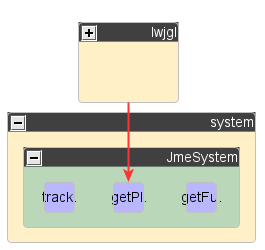
\includegraphics[width=\textwidth]{figures/jme-system-general-part.png}
\caption{The responsibility of this subsystem is handling system related state like a name and platform.}
\label{fig:system-state-incoming}
\end{subfigure}

\caption{The decomposition of JmeSystem. The afferent coupling is reduced to 9.}
\label{fig:system-decomposition}
\end{figure}


% \newpage
\section{Feasibility}
	With an afferent coupling of 21 reported by Sonar, 
	it is not nearly as bad as the Material class (which has an afferent coupling 193).
	However, due to the limited resources we have, refactoring the JmeSystem is actually the
	better choice, as it's a clear violation but still feasible with our resources.

% \newpage
\section{Before}
Before the start of our refactoring, there were only 12 unit tests.
None of which covered the code we planned on refactoring.


% \newpage
\section{After}
We have written 86 test cases in total for the classes JmeSystem, JmeSystemDelegate, JmeDesktopSystem and JmeAndroidSystem.
Together with the 12 testcases that already existed, the testsuite has 98 tests (see Figure~\ref{fig:num-tests}).
This figure shows that we have a single test case with an error.
We did that on purpose, as it exposes a bug in the JmeSystemDelegate, 
where an execution branch can never be visited (equals check of a lowercase string and "PowerPC", see Figure~\ref{fig:bug}).

The testsuite is pretty extensive with an instruction coverage well in the 80\% for the classes under test (see Figures~\ref{fig:cov-core},~\ref{fig:cov-desktop}~and~\ref{fig:cov-android}).
Only JmeDesktopSystem was not covered properly at only 71\%. 
This was due to some missing classes in our project (the Jogl classes),
making it impossible to fully test the class. 
However, those non-covered parts (newContextJogl) are actually almost duplicates (supported by incode code duplicate findings) of pieces that are covered (newContextLwjgl).
So we are still confident that our testsuite suffices.

\begin{figure}[!hb]
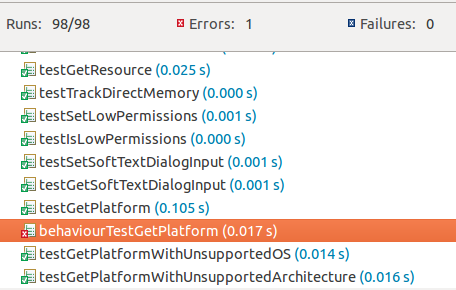
\includegraphics[width=\textwidth]{figures/86-new-tests.png}
\caption{a run of the test suite. Showing 98 testcases and a single failure (indicating the bug of Figure~\ref{fig:bug})}
\label{fig:num-tests}
\end{figure}

\begin{figure}[!hb]
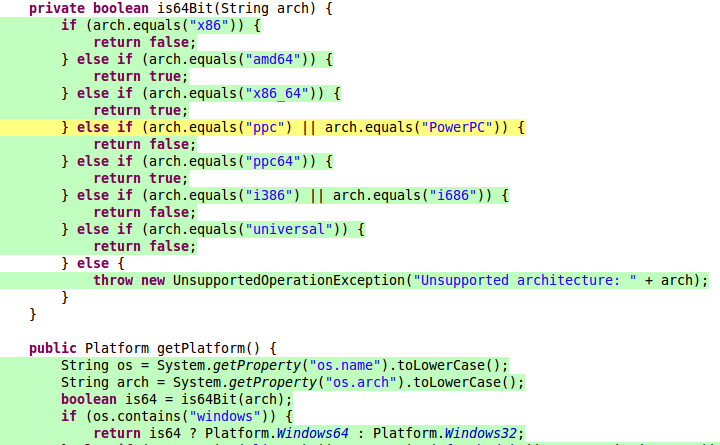
\includegraphics[width=\textwidth]{figures/bug-in-delegate.png}
\caption{The coverage indicates that the branch on matching "PowerPC" is not covered. The only call to is64 actually only passes lowercased strings.}
\label{fig:bug}
\end{figure}

\begin{figure}[!hb]
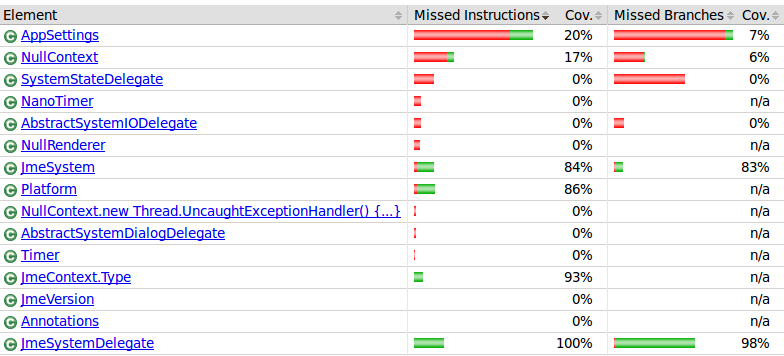
\includegraphics[width=\textwidth]{figures/test-coverage-core.png}
\caption{Test coverage for the com.jme3.system package in the src/core folder. We made testsuites for JmeSystem and JmeSystemDelegate.}
\label{fig:cov-core}
\end{figure}

\begin{figure}[!hb]
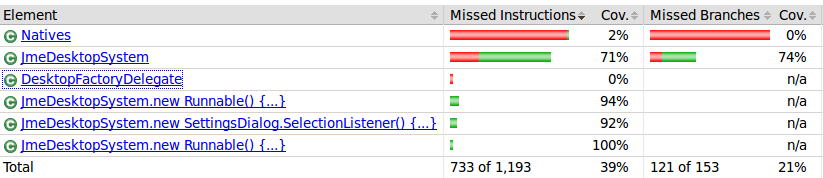
\includegraphics[width=\textwidth]{figures/test-coverage-desktop.png}
\caption{Test coverage for the com.jme3.system package in the src/desktop folder. We made a testsuite for JmeDesktopSystem.}
\label{fig:cov-desktop}
\end{figure}

\begin{figure}
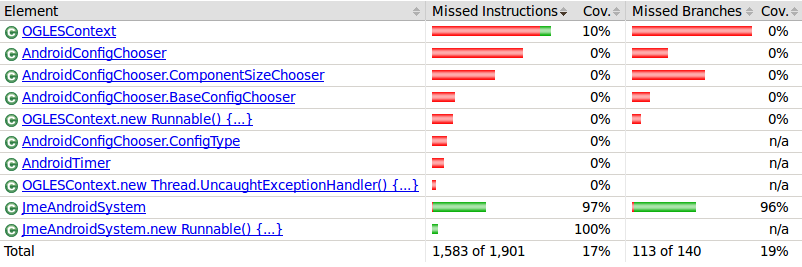
\includegraphics[width=\textwidth]{figures/test-coverage-android.png}
\caption{Test coverage for the com.jme3.system.android package in the src/android folder. We made a testsuite for JmeAndroidSystem.}
\label{fig:cov-android}
\end{figure}

\end{document}
